
\chapter{Ugeopgave 3}
\label{cha:ugeopgave-3}

\section{Part 1}
\begin{itemize}

\item $L_{e}$ er \texttt{GL\_EMISSION} i \texttt{glMaterial*()}
\item $L_{a}$ er \texttt{GL\_AMBIENT} i \texttt{glLight*()}
\item $L_{d}$ er \texttt{GL\_DIFFUSE} i \texttt{glLight*()}
\item $L_{s}$ er \texttt{GL\_SPECULAR} i \texttt{glLight*()}
\item $K_{a}$ er \texttt{GL\_AMBIENT} i \texttt{glMaterial*()}
\item $K_{d}$ er \texttt{GL\_DIFFUSE} i \texttt{glMaterial*()}
\item $K_{s}$ er \texttt{GL\_SPECULAR} i \texttt{glMaterial*()}
\item $l$ er \texttt{GL\_SPOT\_DIRECTION} i \texttt{glLight*()}
\item $\alpha$ er \texttt{GL\_SHININESS} i \texttt{glMaterial*()}

\end{itemize}

Ambient lys simulerer det lille m�ngde lys der bliver spredt over hele scenen.

Fordelen ved 2 \textit{ambient terms} er at der er farve p� objekter i scenen selvom der ikke er sat en lyskilde op, fordi der er et globalt ambient lys.



\section{Part 2}

Programmet kan ses i figur \ref{fig:3-2-1}.

\begin{figure}[hp]
\centering
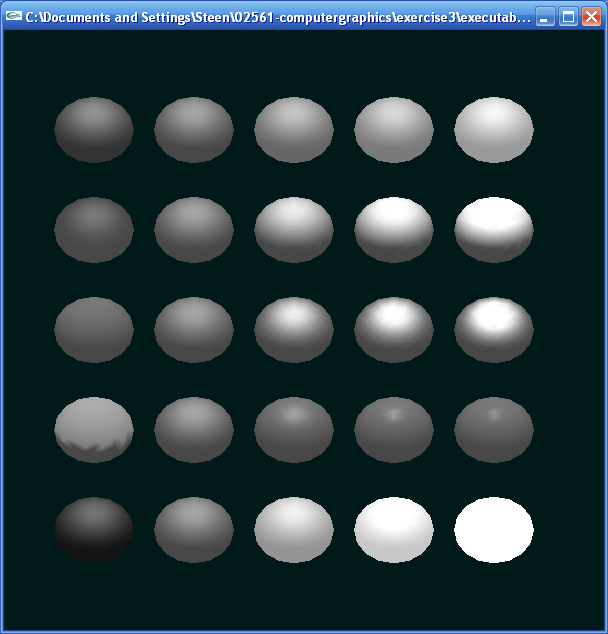
\includegraphics[width=8cm]{../exercise3/screenshots/2.png}
\caption{bolde}
\label{fig:3-2-1}
\end{figure}

Setting the diffusal material to 0,0,0:
Hvis man s�tter diffusal material til 0,0,0 mister kuglen dens genskind p� n�r det der kommer fra det specul�re materiale. Den bryder ikke l�ngere lyset ud i flere vinkler.


Setting the specular material to 0,0,0:
Hvis man s�tter det specular material til 0,0,0 mister man den glas-agtige reflektion og det bliver sv�rere at se hvor lyskilden er placeret i forhold til objektet. Det spekul�re genskind beholder vinklen s� indgangsvinkel er lig udgangsvinkel.

What is the effect of inreasing shininess:
Hvis shininess g�r mod uendeligt n�rmer vi os et spejl. Vi kan se at n�r vi har sat shininess til 0 s� reflekterer kuglen lys i i mange vinkler og ikke koncentreret.

\section{Part 3}

Programmet kan ses i figur \ref{fig:3-3-1}.

\begin{figure}[hp]
\centering
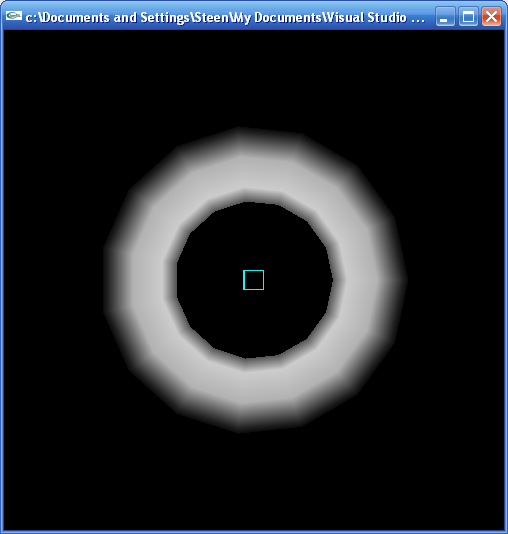
\includegraphics[width=8cm]{../exercise3/screenshots/3.png}
\caption{Torus}
\label{fig:3-3-1}
\end{figure}

Eye point at infinity:
Hvis man flytter eye point til infinity kan nogle beregninger simplificeres. Der er lille forskel mellem vektorerne fra et objekt til �jet n�r man bev�ger sig hen over objektet.

Has the eye point any influence on shading:
Da et objects shading afh�nger af vinklen mellem light sourcen og eye har �jets position meget at sige om shading af et objekt.


Light at infinity:
Hvis man s�tter lyskilden til infinity bliver det et ``directional light'' s� lyset blot kommer fra en side, men ikke nogen vinkel. Det svarer til man har en uendelig stor lampe st�ende i den ene ende af ens univers.

Binding the lightsource to the eye:
Belysningen p� et objekt vil altid komme fra samme punkt som man kigger fra. Det betyder at man aldrig vil se omr�der der ikke bliver belyst.

Using a directional light source:
Hvis man bruger et directional light vil lyset altid komme paralelt fra den bestemte retning.

\section{Part 4}

De 2 shadings kan ses i figur \ref{fig:3-4-1} og \ref{fig:3-4-2}

\begin{figure}[hp]
\centering
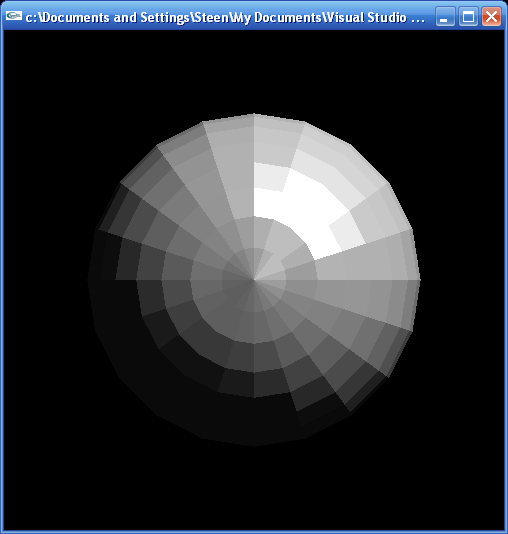
\includegraphics[width=8cm]{../exercise3/screenshots/4-1.png}
\caption{FLAT}
\label{fig:3-4-1}
\end{figure}

\begin{figure}[hp]
\centering
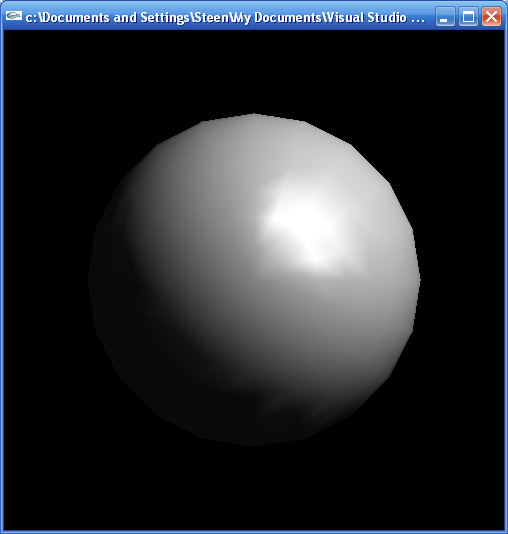
\includegraphics[width=8cm]{../exercise3/screenshots/4-2.png}
\caption{GOURAUD}
\label{fig:3-4-2}
\end{figure}

Difference on Flat, Gouraud and Fong shading:
Flat shading skaber ``Mach bands'' mellem polygoner hvilket vil v�re meget synlige p� runde former.

Gouraud shading behandler vertexerne i et polygon og interpolerer mellem dem, mens Fong shading kan udregne pixel for pixel.


\texttt{Gouraud or Phong for highlighting:} Hvis en highlighting tager
et drastisk fald lige efter en vertex og man bruger Gouraud til at
udregne sin shading vil faldet blive interpoleret og derved spredt ud
gennem polygonet og derved bliver highlightingen st�rere, is�r hvis
der er f� polygoner i ens objekt. Fordi Phong beregner per pixel vil
det v�re bedre at bruge denne.

\texttt{Does Gouraud shading depends on orientation:} Gouraud shading
kan �ndre sig hvis man roterer et objekt. Hvis man har en firkant hvor
2 modst�ende vertexer har v�rdi 1 og de resterende 2 har 0 s� kan man
dele den op p� 2 m�der. Den ene m�de har hvert polygon 2 vertexer med
v�rdi 1, den anden har 2 med v�rdi 0. Hvis man s� interpolerer vil
centrum af kassen f� v�rdi 1 i det ene tilf�lde og v�rdi 0 i det
andet, hvilket giver 2 forskellige resultater.

\section{Part 5}

I figur \ref{fig:3-5-1} ses et billede af animationen hvor lyset flytter sig.

I figur \ref{fig:3-5-2} ses et billede af animationen hvor eye-point flytter sig.

I figur \ref{fig:3-5-3} ses et billede af animationen hvor eye-point og lyset flytter sig uafh�ngigt af hinanden.

I figur \ref{fig:3-5-4} ses et billede af animationen hvor eye-point og lyset flytter sig sammen.

\begin{figure}[hp]
\centering
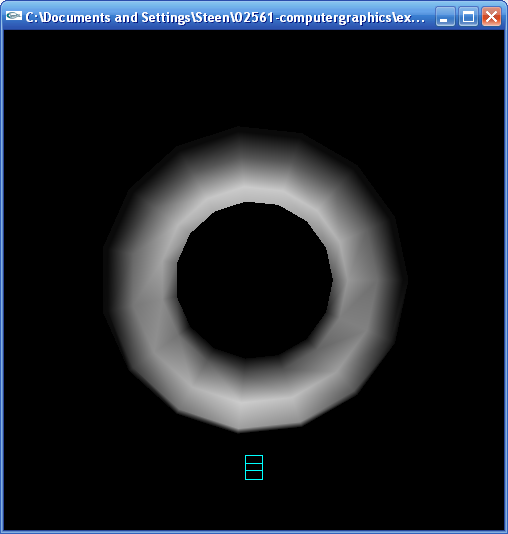
\includegraphics[width=8cm]{../exercise3/screenshots/5-a1.png}
\caption{Moving light}
\label{fig:3-5-1}
\end{figure}
\begin{figure}[hp]
\centering
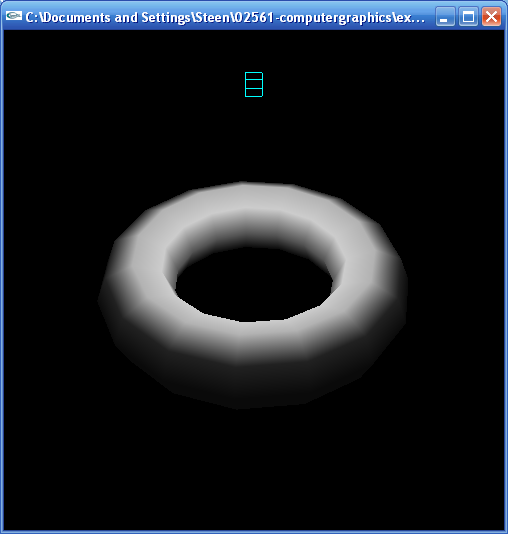
\includegraphics[width=8cm]{../exercise3/screenshots/5-a2.png}
\caption{Moving eye}
\label{fig:3-5-1}
\end{figure}
\begin{figure}[hp]
\centering
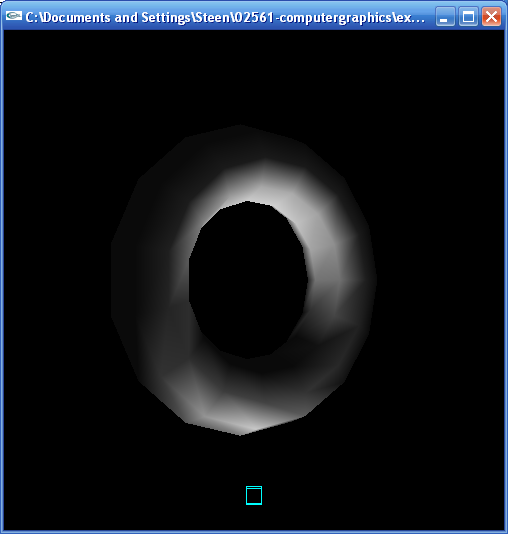
\includegraphics[width=8cm]{../exercise3/screenshots/5-a3.png}
\caption{Moving light and eye, independant}
\label{fig:3-5-1}
\end{figure}
\begin{figure}[hp]
\centering
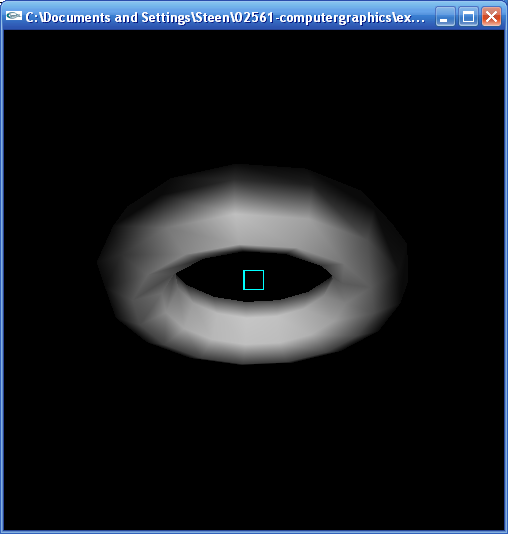
\includegraphics[width=8cm]{../exercise3/screenshots/5-a4.png}
\caption{Moving light and eye, together}
\label{fig:3-5-1}
\end{figure}